\chapter{Lovászova Theta funkce}

\section{Shannonova kapacita}

\subsection*{Definice úlohy}

Představme si komunikační kanál, kterým posíláme zprávy. Tyto zprávy jsou složeny ze symbolů nějaké konečné abecedy. Vlivem šumu mohou být některé symboly druhou stranou špatně interpretovány a naším cílem je vybrat co největší množinu slov délky $k$ tak, aby žádná dvě odeslaná slova nebyla vlivem tohoto šumu zaměnitelná.

Problém si formalizujeme v řeči teorie grafů. Mějme neorientovaný graf $G = (V, E)$, kde množina vrcholů představuje symboly z konečné abecedy a dva vrcholy $x, y$ jsou spojeny hranou, pokud vrchol $x$ může být vlivem šumu zaměněn za $y$.

Maximální počet nezaměnitelných zpráv délky $1$ je roven $\alpha(G)$, kde $\alpha(G)$ značí velikost největší nezávislé množiny v grafu $G$. Pro popis delších zpráv definujeme \textbf{silný součin} $G \cdot H$ grafů $G$ a $H$ následovně
\begin{equation*}
    V(G \cdot H) = V(G) \times V(H),
\end{equation*}
\begin{equation*}
    \begin{split}
    E(G \cdot H) = &\left\{ (i,u)(j,v) \mid ij \in E(G) \wedge uv \in E(H) \right\} \cup \\
                   &\left\{ (i,u)(j,v) \mid ij \in E(G) \wedge u = v \right\} \cup \\
                   &\left\{ (i,u)(j,v) \mid i = j \wedge uv \in E(H) \right\}.
    \end{split}
\end{equation*}

\begin{pr}
Pro graf $P_4 = a-b-c-d-e$ je silný součin $P_4 \cdot P_4$ zobrazen na obrázku~\ref{fig:strong_product_P4_P4}, ze kterého je hezky vidět, že např. zpráva $cd$ (na obrázku červeně) může být zaměněna s $bc$, $bd$, $be$, $cc$, $ce$, $dc$, $dd$ a $de$ (na obrázku oranžově). Podobně pro další zprávy.
\end{pr}

\begin{figure}[h!]
    \centering
    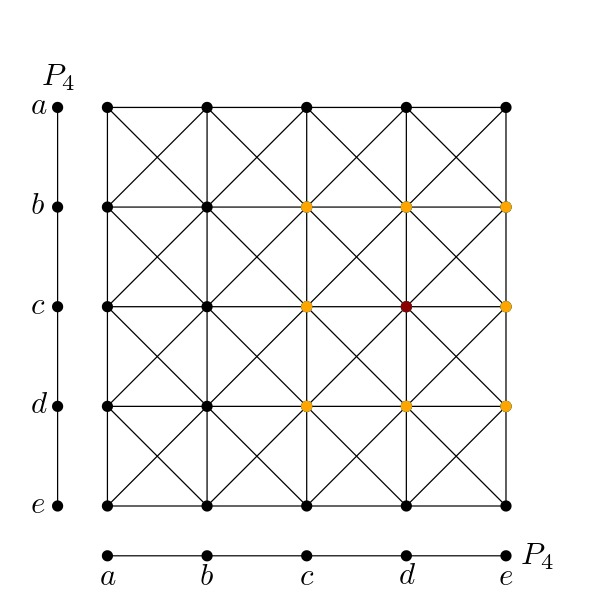
\includegraphics[width=0.5\textwidth]{img/strong_product_P4_P4.png}   
    \caption{$P_4 \cdot P_4$}
    \label{fig:strong_product_P4_P4}
\end{figure}

Pro jednoduchost budeme silný součin $k$ kopií grafu $G$ značit $G^k$. Tedy $\alpha(G^k)$ je maximální počet nezaměnitelných zpráv délky $k$. \textbf{Shannonova kapacita} grafu $G$ je definována jako:
$$
    \Theta(G) = \sup \left\{ \alpha(G^k)^{1/k} \mid k = 1, 2, \dots \right\}.
$$

Neví se, zda pro libovolný graf $G$ existuje vůběc nějaký algoritmus, kterým bychom určili hodnotu $\Theta(G)$. Přesto je alespoň něco známo. Pro perfektní grafy Claude E. Shannon ukázal, že $\Theta(G) = \alpha(G)$. To také znamená, že pro perfektní grafy lze $\Theta(G)$ určit v polynomiálním čase. Dalším kdo se problémem zabýval byl László Lovász, který velmi hezkým způsobem ukázal, že kružnice délky $5$ má kapacitu $\sqrt{5}$. Na Lovászův postup se dále podíváme, protože vede k obecnému hornímu odhadu na $\Theta(G)$.

\subsection*{$\Theta(C_5) = \sqrt{5}$}

Nejprve potřebujeme zavést několik pojmů. \textbf{Tenzorový součin} vektorů $\mathbf{u} = \left(u_1, \dots, u_n \right)$ a $\mathbf{v} = \left(v_1, \dots, v_m \right)$ je
$$
    \mathbf{u} \circ \mathbf{v} = \left( u_1 v_1, \dots, u_1 v_m, u_2 v_1, \dots, u_n v_m \right).
$$

Užitečné bude následující pozorování, které dává do souvislosti skalární a tenzorový součin.

\begin{pz}
    Nechť $\mathbf{x}, \mathbf{u}$ jsou vektory délky $n$ a $\mathbf{y}, \mathbf{v}$ jsou vektory délky $m$. Potom platí
    \begin{equation}
        \left( x \circ y \right)^T \left( u \circ v \right) = \left( x^T u \right) \left( y^T v \right).
        \label{eq:tensor_scalar_product}
    \end{equation}
\end{pz}

\begin{proof}
    Levá strana:
    \begin{equation*}
        \begin{split}
        & \left(x_1 y_1, x_1 y_2, \dots, x_1 y_m, \dots, x_n y_m \right)^T \left( u_1 v_1, u_1 v_2, \dots, u_1 v_m, \dots, u_n v_m \right) = \\
        & x_1 y_1 u_1 v_1 + x_1 y_2 u_1 v_2 + \dots + x_1 y_m u_1 v_m + \dots + x_m y_m u_n v_m
        \end{split}
    \end{equation*}
    Pravá strana:
    \begin{equation*}
        \begin{split}
            & \left( x_1 u_1 + \dots + x_n u_n \right) \cdot \left( y_1 v_1 + \dots + y_n v_m \right) = \\
            & x_1 y_1 u_1 v_1 + x_1 y_2 u_1 v_2 + \dots + x_1 y_m u_1 v_m + \dots + x_m y_m u_n v_m
        \end{split}
    \end{equation*}
\end{proof}

Mějme graf $G = (V,E)$, kde $V = \left\{ 1, \dots, n \right\}$. Systém $\left( \textbf{v}_1, \dots, \textbf{v}_n \right)$ jednotkových vektorů v Euklidovském prostoru takový, že
$$
    \forall ij \notin E \implies \textbf{v}_i \perp \textbf{v}_j
$$
nazýváme \textbf{ortonormální reprezentace} grafu $G$. Poznamenejme, že každý graf má nějakou ortonormální reprezentaci, např. $1 \mapsto \mathbf{e}_1, \dots, n \mapsto \mathbf{e}_n$.

\begin{lm}
    Nechť $\left( \mathbf{u}_1, \dots, \mathbf{u}_n \right)$ je ortonormální reprezentace grafu $G$ a $\left( \mathbf{v}_1, \dots, \mathbf{v}_m \right)$ je ortonormální reprezentace grafu $H$. Potom $\mathbf{u}_i \circ \mathbf{v}_j$ je ortonormální reprezentace grafu $G \cdot H$.
    \label{lemma:shannon}
\end{lm}

\begin{proof}
    Použijeme vztah \ref{eq:tensor_scalar_product}. $\left( u_i \circ v_j \right)^T \left( u_k \circ v_l \right) = \left( u_i^T u_k \right) \left( v_j^T v_l \right) = 0 \iff ik \notin E(G) \vee jl \notin E(H)$.
\end{proof}

\begin{figure}[h!]
    \centering
    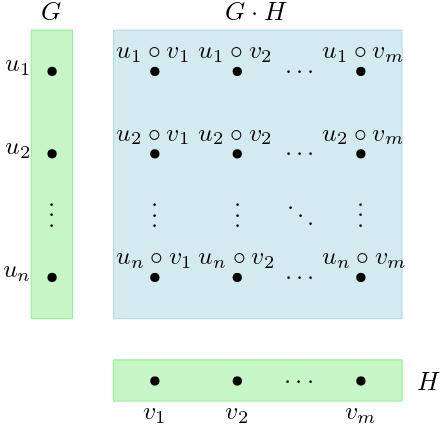
\includegraphics[width=0.5\textwidth]{img/shannon_lemma.png} 
    \caption{Lemma~\ref{lemma:shannon}}
\end{figure}

\noindent \textbf{Hodnotu} ortonormální reprezentace $\left(u_1, \dots, u_n \right)$ definujeme jako
$$
    \min_c \max_{i = 1, \dots, n} \frac{1}{\left( c^T u_i \right)^2}.
$$
Vektoru $c$, pro který nastává minimum říkáme \textbf{handle} dané ortonormální reprezentace.

Dále definujeme funkci $\vartheta(G)$ jako minimální hodnotu přes všechny ortonormální reprezentace grafu $G$. Ortonormální reprezentaci, pro kterou nastává minumum nazýváme \textbf{optimální}. Funkci $\vartheta(G)$ se říká \textbf{Lovászova theta funkce} a ona je právě již zmíněným horním odhadem na $\Theta(G)$. Podívejme se na některé její vlastnosti.

\begin{lm}
    $\vartheta(G \cdot H) \leq \vartheta(G) \vartheta(H)$
\end{lm}

\begin{proof}
    Nechť $\left( u_1, \dots, u_n \right)$ je optimální ortonormální reprezentace grafu $G$ s handle $c$ a $\left( v_1, \dots, v_m \right)$ je optimální ortonormální reprezentace grafu $H$ s handle $d$. Pak $c \circ d$ je jednotkový vektor a platí
    $$
        \vartheta(G \cdot H) \leq \max_{i,j} \frac{1}{\left( \left( c \circ d \right)^T \left( u_i \circ v_j \right) \right)^2} = \max_i \frac{1}{\left( c^T u_i \right)^2} \cdot \max_j \frac{1}{\left( d^T v_j \right)^2} = \vartheta(G)\vartheta(H).
    $$
\end{proof}

\begin{lm}
    $\alpha(G) \leq \vartheta(G)$
\end{lm}

\begin{proof}
    Mějme maximální nezávislou množinu $I \subseteq V(G)$ v grafu $G$ a optimální ortonormální reprezentaci $\mathcal{U} = \left(\mathbf{u}_1, \dots, \mathbf{u}_n \right)$ grafu $G$ s handle $\mathbf{c}$. Platí
    $$
        \forall i,j \in I:\ i \neq j \implies \mathbf{u}_i \bot \mathbf{u}_j.
    $$
    Máme tedy systém ortonormálních vektorů $\left\{ u_i \in \mathcal{U} \mid i \in I \right\}$ v $\mathbb{R}^n$. Ten rozšíříme na ortonormální bázi $\mathcal{B}$. Potom $i$-tá souřadnice vektoru $\mathbf{c}$ v bázi $\mathcal{B}$ je $\mathbf{c}^T \mathbf{u}_i$. Tedy
    $$
        1 = \|\mathbf{c}\|^2 = \sum_{i=1}^n \left( \mathbf{c}^T \mathbf{u}_i \right)^2.
    $$
    Dále vynecháme přidáné vektory do ortonormální báze $\mathcal{B}$
    $$
        \sum_{i=1}^n \left( \mathbf{c}^T \mathbf{u}_i \right)^2 \geq \sum_{i \in I} \left( \mathbf{c}^T \mathbf{u}_i \right)^2.
    $$
    Poslední výraz přepíšeme
    $$
        \sum_{i \in I} \left( \mathbf{c}^T \mathbf{u}_i \right)^2 \geq |I| \cdot \min_{i \in I}\left( \mathbf{c}^T \mathbf{u}_i \right)^2 = \alpha(G) \cdot \min_{i \in I}\left( \mathbf{c}^T \mathbf{u}_i \right)^2.
    $$
    Předchozí výrazy dáme dohromady
    $$
        1 \geq \alpha(G) \cdot \min_{i \in I}\left( \mathbf{c}^T \mathbf{u}_i \right)^2,
    $$
    a dostáváme
    $$
        \alpha(G) \leq \frac{1}{\min_{i \in I}\left( \mathbf{c}^T \mathbf{u}_i \right)^2} = \max_{i \in I} \frac{1}{\left( \mathbf{c}^T \mathbf{u}_i \right)^2} \leq \max_{i \in V(G)} \frac{1}{\left( \mathbf{c}^T \mathbf{u}_i \right)^2} = \vartheta(G).
    $$
\end{proof}

\begin{lm}
    $\Theta(G) \leq \vartheta(G)$
\end{lm}

\begin{proof}
    Pro každé $k$ platí, že
    $$
        \alpha(G^k) \leq \vartheta(G^k) \leq \vartheta(G)^k.
    $$
    Odtud
    $$
        \sqrt[k]{\alpha(G^k)} \leq \vartheta(G),
    $$
    a limitním přechodem dostáváme požadovanou nerovnost
    $$
        \Theta(G) = \lim_{k \to \infty} \sqrt[k]{\alpha(G^k)} \leq \vartheta(G).
    $$
\end{proof}

\begin{vt}
    $\Theta(C_5) = \sqrt{5}$
\end{vt}

\begin{proof}
    Ukážeme konstrukci ortonormální reprezentace grafu $C_5$, ze které dostaneme horní odhad na $\Theta(C_5)$. Nechť $V(C_5) = \left\{ v_1, \dots, v_5 \right\}$ a $E(C_5) = \left\{ v_1v_2, v_2v_3, v_3v_4, v_4v_5, v_1v_5 \right\}$. Mějme vektory $\bar{\mathbf{u}}_i$ ve tvaru
    $$
        \bar{\mathbf{u}}_i = \left( \cos\frac{2 \pi i}{5}, \sin \frac{2 \pi i}{5}, z \right), i = 1, \dots, 5.
    $$
    Každý vektor $\bar{\mathbf{u}}_i$ je svázán s vrcholem $v_i$. Chceme, aby dva vektory, které jsou příslušné nesousedním vrcholům, byly ortogonální. Tedy například $\langle \bar{\mathbf{u}}_2, \bar{\mathbf{u}}_5 \rangle = 0$. Dosadíme
    $$
        \left\langle \bar{\mathbf{u}}_2, \bar{\mathbf{u}}_5 \right\rangle = 
        \left\langle ( \cos\frac{4\pi}{5}, \sin\frac{4\pi}{5}, z ), \left( 1, 0, z \right) \right\rangle =
        \cos\frac{4\pi}{5} + z^2 = 0.
    $$
    Dostáváme tedy
    $$
        z = \sqrt{-\cos\frac{4\pi}{5}}.
    $$
    Definujeme ortonormální reprezentaci $\mathcal{U}$ grafu $C_5$ (projekce do první a druhé souřadnice, viz Obrázek~\ref{fig:umbrella_projection}) tak, že
    $$
        \mathbf{u}_i = \frac{\bar{\mathbf{u}}}{\| \bar{\mathbf{u}} \|}, i = 1, \dots, 5,
    $$
    s handle $\mathbf{c} = \left( 0, 0, 1 \right)$.
    Dostáváme
    $$
        \vartheta(C_5) \leq \vartheta(\mathcal{U}) = \max_{i = 1, \dots, 5} \frac{1}{(\mathbf{c}^T\mathbf{u}_i)^2} = \frac{1}{(\mathbf{c}^T\mathbf{u}_5)^2} = \frac{1 - \cos\frac{4\pi}{5}}{-\cos\frac{4\pi}{5}}.
    $$
    Do posledního výrazu dosadíme známou hodnotu pro $\cos 36^{\circ}$.
    $$
        \frac{1 - \cos\frac{4\pi}{5}}{-\cos\frac{4\pi}{5}} = \frac{1 + \frac{1 + \sqrt{5}}{4}}{\frac{1 + \sqrt{5}}{4}} = \frac{5 + \sqrt{5}}{1 + \sqrt{5}} = \sqrt{5}.
    $$
    Dostáváme
    \begin{equation}
        \vartheta(C_5) \leq \sqrt{5}.
    \end{equation}
    Této ortonormální reprezentaci se říká \textbf{Lovászův deštník}, viz Obrázek~\ref{fig:umbrella}. Druhou nerovnost $\vartheta(C_5) \geq \sqrt{5}$ dostaneme snadno. Sice $\alpha(C_5) = 2$, ale $\alpha(C_5^2) = 5$. Z čehož plyne druhá nerovnost.
\end{proof}

\begin{figure}[h!]
    \centering
    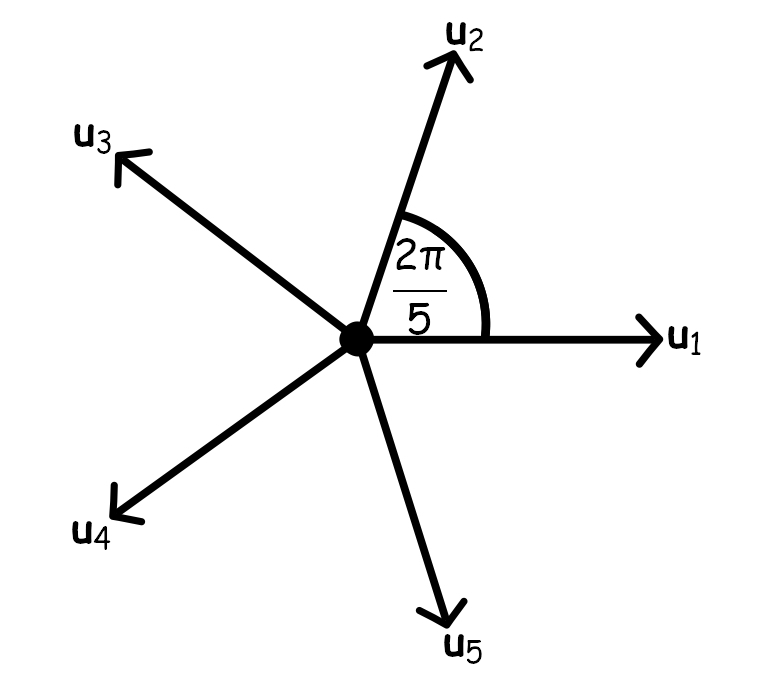
\includegraphics[width=0.5\textwidth]{img/umbrella_projection.png} 
    \caption{Projekce $\mathbf{u}_i$ do první a druhé souřadnice.}
    \label{fig:umbrella_projection}
\end{figure}

\begin{figure}[h!]
    \centering
    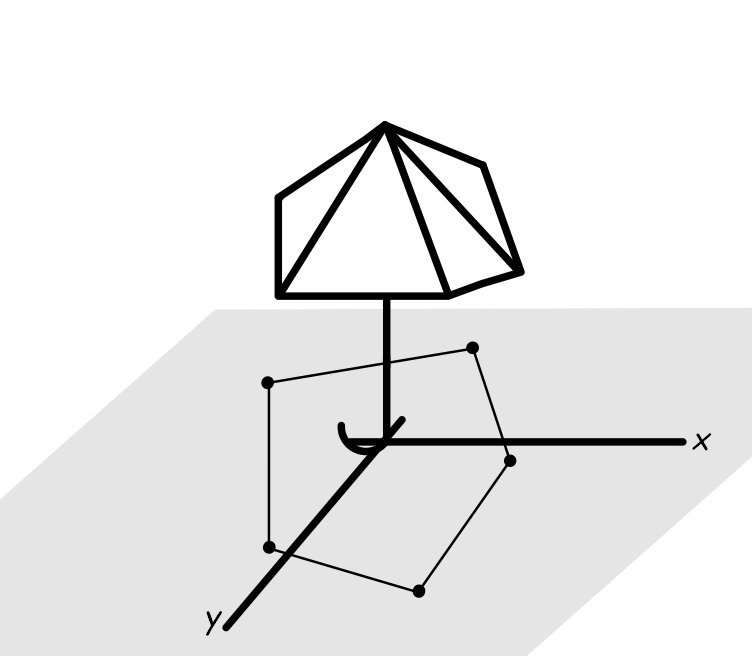
\includegraphics[width=0.5\textwidth]{img/umbrella.png} 
    \caption{Lovászův deštník.}
    \label{fig:umbrella}
\end{figure}


\section{Barvení grafů}
vztah $\vartheta$ k barvení $\overline{G}$, ...


\section{Semidefinitní programy pro $\vartheta(G)$}

formulace / odvození semidefinitních programů pro $\vartheta$ funkci, udělat implementaci
